\documentclass[letterpaper, 10 pt, conference]{ieeeconf}  % Comment this line out if you need a4paper

%\documentclass[a4paper, 10pt, conference]{ieeeconf}      % Use this line for a4 paper

\IEEEoverridecommandlockouts                              % This command is only needed if 
                                                          % you want to use the \thanks command

\overrideIEEEmargins                                      % Needed to meet printer requirements.




% The following packages can be found on http:\\www.ctan.org
\usepackage{graphics} % for pdf, bitmapped graphics files
\usepackage{epsfig} % for postscript graphics files
% \usepackage{times}
% \usepackage{newtxtext,newtxmath} % Times-like text and math fonts

\usepackage{mathptmx} % assumes new font selection scheme installed
\usepackage{times} % assumes new font selection scheme installed
\usepackage{amsmath} % assumes amsmath package installed
\usepackage{amssymb}  % assumes amsmath package installed
% \usepackage[utf8]{inputenc}

\usepackage{cite} % Use cite.sty for numerical citation management
\usepackage[bookmarks=true]{hyperref} % Use hyperref for other links
% \usepackage{hyperref} % Use hyperref for other links
% \usepackage{appendix}

\usepackage{tikz}
\usepackage{float}
\usepackage{svg}
% \usepackage{bm}
\usepackage{balance}

\tikzstyle{block} = [rectangle, minimum width=2cm, minimum height=1cm,text centered, draw=black]
\tikzstyle{block_1} = [rectangle, minimum width=2cm, minimum height=1cm,text centered, draw=black, fill=blue!5]
\tikzstyle{block_2} = [rectangle, minimum width=2cm, minimum height=1cm,text centered, draw=black, fill=red!5]
\tikzstyle{arrow} = [thick,->,>=stealth]
\tikzstyle{arrow_2} = [very thick,->,>=stealth]
\tikzstyle{arrow_3} = [thick,->,>=stealth,dashed]
\tikzstyle{pfr} = [cylinder, draw, minimum height=4cm, minimum width=1cm, shape aspect=1, shape border rotate=180]
\usetikzlibrary{shapes.geometric}


% Override the fake natbib command to allow cite.sty and hyperref to work together
\makeatletter
\let\NAT@parse\undefined
\makeatletter

\title{\LARGE \bf
Observer-based MPC of an Axial Dispersion Tubular Reactor:\\ Addressing Recycle Delays through Transport PDEs
}


\author{Behrad Moadeli and Stevan Dubljevic$^{1}$% <-this % stops a space
\thanks{$^{1}$Behrad Moadeli and Stevan Dubljevic are with the Department of Chemical and Materials Engineering,
University of Alberta, Edmonton, AB, Canada T6G 1H9
{\tt\small moadeli@ualberta.ca}, {\tt\small stevan.dubljevic@ualberta.ca}}%
\thanks{Funding provided by the Natural Sciences and Engineering Research Council of Canada—NSERC (RGPIN-2022-03486).}% <-this % stops a space
}


\begin{document}



\maketitle
\thispagestyle{empty}
\pagestyle{empty}


%%%%%%%%%%%%%%%%%%%%%%%%%%%%%%%%%%%%%%%%%%%%%%%%%%%%%%%%%%%%%%%%%%%%%%%%%%%%%%%%
\begin{abstract}

        The model predictive control of an axial dispersion tubular reactor equipped with a recycle stream is presented. The intrinsic time delay imposed by the recycle stream, an often overlooked aspect in chemical engineering process control studies, is modeled as a transport PDE, leading to a boundary-controlled system of coupled parabolic and hyperbolic PDEs under Danckwerts boundary conditions, suitable for this reactor type. Considering the digital nature of controllers, a discrete-time linear model predictive controller is designed to stabilize the system, coupled with a Luenberger state estimator to address the controller's limited access to the system's full state. The need for model reduction through spatial approximation is eliminated by following a late lumping approach, while utilizing Caley-Tustin time discretization method to preserve the continous-time system's characteristics. The controller's effectiveness is demonstrated through numerical simulations, showcasing its capability to stabilize an unstable system while adhering to input constraints, having access merely to output measurements.

\end{abstract}

\section{Introduction}

Many processes in the chemical and petrochemical sectors involve states that evolve over space and time, commonly represented by partial differential equations (PDEs) as distributed parameter systems (DPS) \cite{ray1981advanced}. The infinite-dimensional nature of DPSs presents specific challenges in control and estimation, making this a prominent area of research. Two main methods are often applied to control DPSs: \textit{Early Lumping} and \textit{Late Lumping}. Early Lumping reduces the system to a finite-dimensional approximation through spatial discretization early in the modeling stage, allowing for the application of standard control techniques \cite{davison1976robust}. However, this method can lead to inaccuracies due to mismatches between the reduced model and the original system dynamics \cite{moghadam2012infinite}. Late Lumping, by contrast, preserves the system’s infinite-dimensional structure until the final stages of controller implementation, resulting in a control approach that is more complex but achieves greater fidelity to the original dynamics.

A range of studies in chemical engineering have applied the late lumping method to control infinite-dimensional systems, specifically targeting convection-reaction processes governed by first-order hyperbolic PDEs and diffusion-convection-reaction processes described by second-order parabolic PDEs.
In \cite{christofides1996feedback}, the robust control of first-order hyperbolic PDEs is explored, demonstrating the stabilization of a plug flow reactor system using a distributed input.
A boundary feedback stabilization approach using the backstepping method is presented in \cite{krstic2008backstepping} for a comparable system of first-order hyperbolic PDEs.
The work in \cite{xu2016state} introduces a state feedback regulator design for a countercurrent heat exchanger system, providing another example of a chemical engineering DPS governed by first-order hyperbolic PDEs, distinct from tubular reaction systems.
Highlighting the role of dispersion in axial dispersion tubular reactors, \cite{christofides1998robust} examines the robust control of diffusion-convection-reaction systems governed by second-order parabolic PDEs.
In \cite{dubljevic2006predictive2}, a late-lumping approach is employed to develop a low-dimensional predictive controller for a diffusion-convection-reaction system, utilizing modal decomposition to capture the system's dominant modes.
A similar method is applied in \cite{khatibi2021model} to design an observer-based model predictive controller (MPC) for an axial dispersion tubular reactor, accounting for the impact of recycle streams, a common feature in industrial chemical reactors.
Different aspects of state reconstruction for DPSs are addressed in several works where the design of a discrete-time Luenberger observer is adressed for the class of DPSs, where no spatial discretization is required; a key feature of the late lumping approach  \cite{dochain2000state, dochain2001state, alonso2004optimal, ali2015review}.
%%% ta inja
Delay systems are another class of infinite-dimensional systems that have been studied in the literature \cite{curtainbook}. 
Commonly represented in the form of delay differential equations (DDEs), delay can also be modeled as a transport PDE, showing to be advantageous in more complex scenarios \cite{krstic2009book}. In the field of control theory for chemical engineering DPSs, input/output delay has been addressed in several works as both output measurement delays and input actuation delays are common in industrial processes. 
In general, such delays can be addressed by considering a transportation lag block at either the input or output of the system, resulting in a cascade PDE system \cite{Hiratsuka1969IEEE, mohammadi2012lq, Guilherme2019ACC}. In contrast to input/output delays, state delay is less addressed in the relevant literature, probably since not many applications in this field can be described by state delays. In one of the few attempts, a delayed-state distributed parameter system is addressed in \cite{ozorio2019heat}, where a full-state and output feedback regulator is designed for a system of heat exchangers. The state delay in this works comes from the time it takes for a stream to leave one pass of the heat exchanger and enter the next pass. Similarly in \cite{qi2021output}, a tubular reactor system is considered, where the state delay is introduced as a result of the recycle delay in the system, without considering the diffusion term along the reactor. Even in \cite{khatibi2021model} where the recycle stream is considered for a distributed diffusion-convection-reaction system, the recycle is assumed to be instantaneous; a simplifying assumption that leaves a gap in the literature regarding diffusion-convection-reaction systems with a recycle stream imposing state delay.

In this work, an axial dispersion tubular reactor equipped with recycle is addressed as a diffusion-convection-reaction DPS. First, the reactor is modeled by a second order parabolic PDE, where the recycle stream poses a state delay, resulting in a first order hyperbolic transport PDE coupled with the original PDE. Late lumping approach is utilized by obtaining the resolvent of the infinite-dimensional system in a closed operator form, with no need to perform spatial discretization. Then, to enable the implementation of MPC as a digital controller, discrete-time representation of the system is obtained using Caley-Tustin time discretization technique; i.e. a Crank-Nicolson type of discretization that preserves the conservative characteristics of the continuous system, mitigating the need for model reduction \cite{havu2007cayley, xu2017linear}. Finally via numerical simulations, the proposed controller is shown to stabilize an unstable system within an optimal framework, given input constraints.
\section{Continuous-time Model Representation}

Fig.~\ref{fig:reactor_scheme} illustrates a chemical process, i.e. a first-order irreversible reaction within an axial dispersion tubular reactor \cite{levenspiel1998chemical}. The reactor is equipped with a recycle mechanism, allowing a portion of the product stream to re-enter the reactor, increasing the conversion of the substrate.  Utilizing first-principle modeling through relevant mass balance relations on an infinitesimally thin disk element along the longitudinal axis of the reactor, the dynamics describing the concentration within the system results in a second-order parabolic PDE, a common class of equations used to characterize diffusion-convection-reaction systems \cite{jensen1982bifurcation}. 

\begin{figure}[!htbp] 
    \centering
    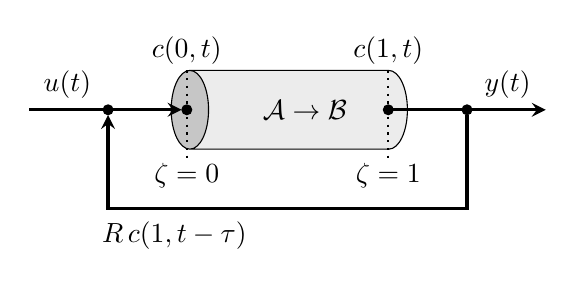
\begin{tikzpicture}
        \node (pfr) [cylinder, draw, minimum height=3cm, minimum width=1cm, shape aspect=1, shape border rotate=180, cylinder uses custom fill, cylinder end fill=gray!45, cylinder body fill=gray!15] {$\mathcal{A} \rightarrow \mathcal{B}$};
        \node (pfr_inlet) [circle, left of=pfr, xshift=-0.5cm, fill=black, draw, inner sep=0pt, minimum size=0.25cm, scale=0.5] {};
        \node (pfr_outlet) [circle, at={(pfr.east)}, shift={(-0.25cm,0)}, fill=black, draw, inner sep=0pt, minimum size=0.25cm, scale=0.5] {};
        \node (recycle_right) [circle, right of=pfr_outlet, fill=black, draw, inner sep=0pt, minimum size=0.25cm, scale=0.5] {};
        \node (recycle_left) [circle, left of=pfr_inlet, fill=black, draw, inner sep=0pt, minimum size=0.25cm, scale=0.5] {};
        
        \draw[dotted, thick] ([yshift=0.5cm]pfr_inlet.center) -- node[at end, below, yshift=0.1cm] {$\zeta = 0$} ([yshift=-0.65cm]pfr_inlet.center);
        \draw[dotted, thick] ([yshift=0.5cm]pfr_outlet.center) -- node[at end, below, yshift=0.1cm] {$\zeta = 1$} ([yshift=-0.65cm]pfr_outlet.center);
        
        \node[below of=recycle_left, node distance=1.3cm, anchor=north west, xshift=-0.2cm] {$R \, c(1, t-\tau)$};
        \node[above of=pfr_inlet, node distance=0.75cm,] {$c(0, t)$};
        \node[above of=pfr_outlet, node distance=0.75cm,] {$c(1, t)$};
        
        \draw [arrow_2] (pfr_outlet) -- node[near end, above] {$y(t)$} ++(2,0);
        \draw [arrow_2] (pfr_inlet) ++(-2,0) coordinate(start) -- node[near start, above] {$u(t)$} (pfr_inlet);
        \draw [arrow_2] (recycle_right) -- ++(0,-1.25) -| (recycle_left);
        
    \end{tikzpicture}
    \caption{Axial tubular reactor with recycle stream.}
    \label{fig:reactor_scheme}
    % \pdfbookmark[2]{Figure: Reactor Scheme}{fig:reactor_scheme}
\end{figure}

In an attempt to make the model more realistic for common axial dispersion tubular reactors in chemical industry, Dankwerts boundary conditions are chosen as they are known to be suitable for this purpose by accounting for deviations from perfect mixing and piston flow, assuming negligible transport lags in connecting lines \cite{danckwerts1993continuous}. The delayed state resulting from the recycled portion of the flow, occurring $\tau$ seconds back in time, is applied at the inlet boundary condition. The governing equation is given by the PDE represented by \eqref{eq:PDE_original_model}, subject to the abovementioned boundary conditions in \eqref{eq:BC}.

\begin{equation} \label{eq:PDE_original_model}
    \dot{c}(\zeta, t) = D \partial_{\zeta \zeta} c(\zeta, t) - v \partial_\zeta c(\zeta, t) + k_r c(\zeta, t)
\end{equation}

\begin{align} \label{eq:BC}
    \begin{cases}
        &D \partial_\zeta c(0, t) - v c(0, t) = -v \left[ R c(1, t-\tau) + (1-R) u(t) \right] \\
        &\partial_\zeta c(1, t) = 0 \\
        &y(t) = c(1, t)
    \end{cases}
\end{align}

Here, $c(\zeta, t)$ is the concentration of the product along the reactor, representing the state of the system. The physical parameters $D$, $v$, $k_r$, $R$, and $\tau$ represent the diffusion coefficient, flow velocity along the reactor, reaction constant, recycle ratio, and residence time of the recycle flow, respectively. The coordinate system in space and time is represented by $\zeta$ and $t$, where $\zeta \in [0, 1]$ and $t \in [0, \infty)$.

An interesting approach to address delays where the problem involves other forms of PDEs is to reformulate the problem such that the notion of delay is replaced with an alternative transport PDE \cite{krstic2009book}. 
Therefore, the state variable $c(\zeta,t)$ is replaced with a new state variable $\underline{x}(\zeta, t) \equiv [x_1(\zeta, t), x_2(\zeta, t)]^T$ as a vector of functions, where $x_1(\zeta, t)$ represents the concentration within the reactor—analogous to $c(\zeta,t)$—and $x_2(\zeta, t)$ is the new state variable for the concentration along the recycle stream. The delay is thus modeled as a pure transport process rather than being present in the argument of the state at the boundary—i.e. $c(1,t-\tau)$— making all state variables expressed explicitly at a specific time instance $t$, resulting in the standard state-space form for a given infinite-dimensional linear time-invariant (LTI) system $\dot{\underline{x}} = \mathfrak{A} \underline{x} + \mathfrak{B} u$ . Here, $\mathfrak{A}$ is a linear operator $\mathcal{L}(X)$ acting on a Hilbert space $X: L^2[0,1] \times L^2[0,1]$ and $\underline{x}(\zeta,t)$, as defined previously, is the vector of functions describing the states of the system. The operator $\mathfrak{A}$ and its domain are defined in detail as shown in \eqref{eq:operator_A}. Also, $\mathfrak{B}$ is a linear operator that maps the scalar input from input-space onto the state space, as defined in \eqref{eq:operator_B}. Finally, the output operator $\mathfrak{C}$ is defined in \eqref{eq:operator_C}, where the output $y(t)$ is the concentration at the reactor outlet.

\begin{equation} \label{eq:operator_A}
    \begin{aligned}
        \mathfrak{A} \equiv&
        \begin{bmatrix}
            D \partial_{\zeta \zeta} - v \partial_\zeta + k_r & 0 \\
            0 & \frac{1}{\tau} \partial_\zeta
        \end{bmatrix}\\
        \mathcal{D}(\mathfrak{A}) =& \Bigl\{ \underline{x}(\zeta) = [x_1(\zeta), x_2(\zeta)]^T \in X:\\
        &\underline{x}(\zeta), \partial_\zeta \underline{x}(\zeta), \partial_{\zeta \zeta} \underline{x}(\zeta) \quad \mathrm{a.c.},\\
        &D \partial_\zeta x_1(0) - v x_1(0) = -v R x_2(0),\\
        &\partial_\zeta x_1(1) = 0,
        x_1(1) = x_2(1) \Bigr\}
    \end{aligned}
\end{equation}

\begin{equation} \label{eq:operator_B}
    \begin{aligned}
        \mathfrak{B} &\equiv
        \begin{bmatrix}
            \delta(\zeta) \\
            0
        \end{bmatrix} \cdot (1-R) v \\
        % \mathcal{D}(\mathfrak{B}) &= \Bigl\{ u \in \mathbb{R} \Bigr\}
    \end{aligned}
\end{equation}

\begin{equation} \label{eq:operator_C}
    \begin{aligned}
        \mathfrak{C} &\equiv
        \begin{bmatrix}
            \delta(\zeta-1) &
            0
        \end{bmatrix}\\
        % \mathcal{D}(\mathfrak{C}) &= \mathcal{D}(\mathfrak{A})
    \end{aligned}
\end{equation}

with $\delta(\zeta)$ being dirac delta function. The system's spectrum can now be obtained by solving the eigenvalue problem for the system generator $\mathfrak{A}$. To do this, the characteristics equation of the system needs to be obtained by solving the equation $det(\mathfrak{A}-\lambda_i~I)~=~0$ for $\lambda_i$, where $\lambda_i \in \mathbb{C}$ is the $i^{\text{th}}$ eigenvalue of the system and $I$ is the identity operator. Attempts to analytically solve this equation will fail; therefore, it is solved numerically given the parameters in Table~\ref{tab:pars}. The eigenvalue distribution is given in Figure~\ref{fig:eigval_dist} in the complex plane. This suggests that the open-loop system is unstable, as there are eigenvalues with positive real parts.

\begin{figure}[!htbp]
    \centering
    \includesvg[inkscapelatex=false, width=0.35\textwidth, keepaspectratio]{Figures/eig_val_dist_R_0.3.svg}
    \caption{Eigenvalues of operator $\mathfrak{A}$.}
    \label{fig:eigval_dist}
\end{figure}


\begin{table}[ht]
    \centering
    \caption{Physical Parameters for the System}
    \label{tab:pars}
    \begin{tabular}{|c|c|c|c|}
    \hline
    \textbf{Parameter}        & \textbf{Symbol} & \textbf{Value}     & \textbf{Unit}    \\ \hline
    Diffusivity               & $D$             & $2\times10^{-5}$   & ${m^2}/{s}$      \\ \hline
    Velocity                  & $v$             & $0.01$   & ${m}/{s}$        \\ \hline
    Reaction Constant         & $k_r$           & $1.5$              & $s^{-1}$         \\ \hline
    Recycle Residence Time    & $\tau$          & $80$               & $s$              \\ \hline
    Recycle Ratio             & $R$             & $0.3$              & $-$              \\ \hline
    \end{tabular}
\end{table}

It is necessary to obtain the adjoint system operators $\mathfrak{A}^*$ and $\mathfrak{B}^*$ in order to derive the resolvent operator of the system, which is later utilized in performing the Caley-Tustin time discretization. The derivation of the adjoint system operators is provided in Appendix \ref{app:adjoint}, followed by the derivation of an exact closed-form representation for the resolvent operator detailed in Appendix \ref{app:resolvent}. 
\section{Cayley-Tustin Time Discretization}
Having access to the resolvent operators of the original and the adjoint system, the Cayley-Tustin time-discretization can be utilized to map the continuous-time setting to the discrete-time setting without losing crucial dynamical properties of the system, such as stability and controllability. This Crank-Nicolson type of discretization is also known as the lowest order symplectic integrator in Gauss quadrature-based Runge-Kutta methods \cite{hairer2006geometric}. Considering $\Delta t$ as the sampling time, and assuming a piecewise constant input within time intervals (a.k.a. zero-order hold), the discrete-time representation $\underline{x}(\zeta, k) = \mathfrak{A}_d \underline{x}(\zeta, k-1) + \mathfrak{B}_d u(k)$ is obtained, with discrete-time operators $\mathfrak{A}_d$ and $\mathfrak{B}_d$ defined in \eqref{eq:discrete_AB}, where $\alpha = 2/{\Delta t}$. As required for systems with nonself-adjoint generators, the adjoint discrete-time operators $\mathfrak{A}_d^*$ and $\mathfrak{B}_d^*$ are also obtained in a similar manner.
\begin{equation} \label{eq:discrete_AB}
    \begin{bmatrix}
        \mathfrak{A}_d & \mathfrak{B}_d \\
        \mathfrak{C}_d & \mathfrak{D}_d
    \end{bmatrix} = 
    \begin{bmatrix}
        -I + 2\alpha \mathfrak{R}(\alpha, \mathfrak{A}) & \sqrt{2\alpha} \mathfrak{R}(\alpha, \mathfrak{A}) \mathfrak{B}\\
        \sqrt{2\alpha} \mathfrak{C} \mathfrak{R}(\alpha, \mathfrak{A}) & \mathfrak{C} \mathfrak{R}(\alpha, \mathfrak{A}) \mathfrak{B}
    \end{bmatrix}
\end{equation}
\section{Observer Design}

One important issue of DPSs is the limitted access to the states of the infinite-dimensional system as the state is distributed over the entire domain and performing infinite measurements is never feasible. Therefore, an observer is required to estimate the states of the system based on the available measurements. To address this issue, a Luenberger observer is designed to reconstruct the states of the system based on the output measurements. First, the consinuous-time observer design is considered; followed by the design of the discrete-time observer.

\subsection{Continuous-Time Observer Design}

For the purpose of state recunstruction of a diffusion-convection-reaction system, where the feedforward term $\mathfrak{D}$ is generally absent, the continuous-time observer dynamics are given by \eqref{eq:observer_continuous}.

\begin{equation} \label{eq:observer_continuous}
    \begin{aligned}
        \dot{\hat{x}}(\zeta, t) &= \mathfrak{A} \hat{x}(\zeta, t) + \mathfrak{B} u(t) + \mathfrak{L}_c [y(t) - \hat{y}(t)] \\
        \hat{y}(t) &= \mathfrak{C} \hat{x}(\zeta, t)
    \end{aligned}
\end{equation}

where $\hat{x}(\zeta, t)$ is the reconstructed state of the original system and $\mathfrak{L}_c$ is the continuous-time observer gain. By subtracting the observer dynamics from the original system dynamics, the error dynamics $e(\zeta,t$) are obtained as shown in \eqref{eq:observer_error_continuous}.

\begin{equation} \label{eq:observer_error_continuous}
    \begin{aligned}
        \dot{e}(\zeta, t) &= (\mathfrak{A} - \mathfrak{L}_c \mathfrak{C}) e(\zeta, t) \equiv \mathfrak{A}_o e(\zeta,t) \\
    \end{aligned}
\end{equation}

The goal is to design the observer gain $\mathfrak{L}_c$ such that the error dynamics are exponentially stable, i.e. $\max\{\operatorname{Re}(\lambda_{o})\}~<~0$ where $\lambda_{o}$ are the eigenvalues of the error dynamics matrix $\mathfrak{A}_o$. Three different forms of the observer gain are considered as spatial functions $\mathfrak{L}_c = f(\zeta, l_{obs})$ with the effect of the scalar coefficient $l_{obs}$ on $\max\{\operatorname{Re}(\lambda_{o})\}$ shown in Fig.~\ref{fig:L_vs_lambda}.

\begin{figure}[!htbp]
    \centering
    \includesvg[inkscapelatex=false, width=0.42\textwidth, keepaspectratio]{figures/obs_lambda.svg}
    \caption{The effect of various observer gains $\mathfrak{L}_c = f(\zeta, l_{obs})$ on the eigenvalues of state reconstruction error dynamics $\lambda_o$.}
    \label{fig:L_vs_lambda}
\end{figure}


\subsection{Discrete-Time Observer Design}

Once an appropriate continuous-time observer gain is determined, the discrete-time observer gain $\mathfrak{L}_d$ may be obtained using the same Caley-Tustin time discretization approach, as shown in \eqref{eq:observer_discrete}.

\begin{equation} \label{eq:observer_discrete}
    \begin{aligned}
        \hat{x}(\zeta, k) &= \mathfrak{A}_d \hat{x}(\zeta, k-1) + \mathfrak{B}_d u(k) + \mathfrak{L}_d [y(k) - \hat{y}(k)] \\
        \hat{y}(k) &= \mathfrak{C}_{d,o} \hat{x}(\zeta, k-1) + \mathfrak{D}_{d,o} u(k) + \mathfrak{M}_{d,o} y(k)
    \end{aligned}
\end{equation}

with $\mathfrak{A}_d$ and $\mathfrak{B}_d$ defined in \eqref{eq:discrete_AB}, and $\mathfrak{C}_{d,o}$, $\mathfrak{D}_{d,o}$, $\mathfrak{M}_{d,o}$, and $\mathfrak{L}_d$ are given in \eqref{eq:observer_discrete_CDLM}.

\begin{equation} \label{eq:observer_discrete_CDLM}
    \begin{aligned}
        \mathfrak{C}_{d,o} (\cdot) &= \sqrt{2\alpha} \left[ I + \mathfrak{C} (\alpha I - \mathfrak{A}) \mathfrak{L}_c \right]^{-1} \mathfrak{C} \mathfrak{R}(\alpha, \mathfrak{A}) (\cdot) \\
        \mathfrak{D}_{d,o} &= \left[ I + \mathfrak{C} (\alpha I - \mathfrak{A}) \mathfrak{L}_c \right]^{-1} \mathfrak{C} \mathfrak{R}(\alpha, \mathfrak{A}) \mathfrak{B} \\
        \mathfrak{M}_{d,o} &= \left[ I + \mathfrak{C} (\alpha I - \mathfrak{A}) \mathfrak{L}_c \right]^{-1} \mathfrak{C} \mathfrak{R}(\alpha, \mathfrak{A}) \mathfrak{L}_c \\
        \mathfrak{L}_d &= \sqrt{2\alpha} \mathfrak{R}(\alpha, \mathfrak{A}) \mathfrak{L}_c \\
    \end{aligned}
\end{equation}

It has been proven that using this approach, the discrete-time error dynamics will be stable if the continuous-time observer gain $\mathfrak{L}_c$ is chosen such that $\mathfrak{A}_o$ is stable. It is worth noting that the methodology presented skips the need for model reduction associated with the discrete-time Luenberger observer, with no spatial approximation required as well \cite{dochain2000state,dochain2001state,alonso2004optimal,ali2015review,khatibi2021model}.
\section{Model Predictive Controller Design}
In this section, the observer-based MPC shown in Fig.~\ref{fig:block_diagram} is developed with the goal of stabilizing the given unstable infinite-dimensional system within an optimal framework, relying solely on output measurements while satisfying input constraints. 
An infinite-time open-loop objective function sets the foundation of the controller design in the discrete-time setting at each sampling instant $k$. The objective function consists of a weighted sum of actuation costs as well as state deviations, for all future time instances, subject to the system dynamics and input constraints. Since full-state is assumed to be unavailable, reconstructed states are used to estimate states of the system, as shown in \eqref{eq:MPC_inf_time}.
\begin{figure}[!htbp]
    \centering
    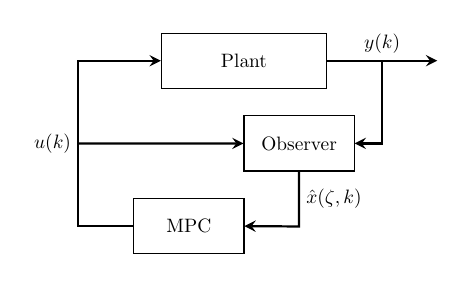
\begin{tikzpicture}[node distance=2cm, scale=0.7, transform shape]
        \node (plant) [block, minimum width=3cm] {Plant};
        \node (regulator) [block, below of=plant, xshift=-1cm, yshift=-1cm] {MPC};
        \node (observer) [block, below of=plant, xshift=1cm, yshift=0.5cm] {Observer};
        \draw [arrow] (plant.east) -- node[midway, above] {$y(k)$} ++(2,0);
        \draw [arrow] (plant.east) ++(1,0) |- (observer.east);
        \draw [arrow] (observer.south) -- ++(0,-1) node[midway, right] {$\hat{{x}}(\zeta,k)$} -- (regulator.east);    
        \draw [arrow] (regulator.west) -- ++(-1,0) |- (plant.west);
        \draw [arrow] (regulator.west) ++(-1,1.5) coordinate(start) -- node[near start, left, xshift=-0.75cm] {$u(k)$} (observer.west);
    \end{tikzpicture}
    \caption{Block diagram representation of the observer-based MPC.}
    \label{fig:block_diagram}
\end{figure}

\begin{equation} \label{eq:MPC_inf_time}
    \begin{aligned}
        \min_{U} \quad \sum_{l=0}^{\infty} &\langle \underline{\hat{x}}(\zeta, k+l | k), \mathfrak{Q} \underline{\hat{x}}(\zeta, k+l | k) \rangle \\
        + &\langle u(k+l+1 | k), \mathfrak{F} u(k+l+1|k) \rangle \\
        \, \\
        \text{s.t.} \quad &\underline{\hat{x}}(\zeta, k+l | k) = \mathfrak{A}_d \underline{\hat{x}}(\zeta, k+l-1 | k) + \mathfrak{B}_d u(k+l | k) \\
        &u^{min} \leq u(k+l | k) \leq u^{max}
    \end{aligned}
\end{equation}
where $\mathfrak{Q}$ and $\mathfrak{F}$ are positive definite operators of appropriate dimensions, responsible for penalizing state deviations and actuation costs, respectively. The notation $(k+l|k)$ indicates the future time states or input instance $k+l$ obtained at time $k$. The infinite-time optimization problem may be reduced to a finite-time setup by assigning zero-input beyond a certain control horizon $N$, resulting in the optimization problem in \eqref{eq:MPC_finite_time}.
\begin{equation} \label{eq:MPC_finite_time}
    \begin{aligned}
        \min_{U} \quad \sum_{l=0}^{N-1} &\langle \underline{\hat{x}}(\zeta, k+l | k), \mathfrak{Q} \underline{\hat{x}}(\zeta, k+l | k) \rangle \\
        + &\langle u(k+l+1 | k), \mathfrak{F} u(k+l+1|k) \rangle \\
        + &\langle \underline{\hat{x}}(\zeta, k+N | k), \mathfrak{P} \underline{\hat{x}}(\zeta, k+N | k) \rangle \\
        \, \\
        \text{s.t.} \quad &\underline{\hat{x}}(\zeta, k+l | k) = \mathfrak{A}_d \underline{\hat{x}}(\zeta, k+l-1 | k) + \mathfrak{B}_d u(k+l | k) \\
        &u^{min} \leq u(k+l | k) \leq u^{max} \\
        & \langle \underline{\hat{x}}(\zeta, k+N | k), \underline{\phi_u}(\zeta) \rangle = 0
    \end{aligned}
\end{equation}
where $\mathfrak{P}$ is the terminal cost operator obtained as the solution to the discrete-time Lyapunov equation, as shown in \eqref{eq:terminal_cost}. This operator can be shown to be positive definite only if the terminal state $\underline{\hat{x}}(\zeta, k+N | k)$ is in a stable subspace. Therefore, for the resulting quadratic optimization problem to be convex, an equality constraint is introduced to guarantee $\mathfrak{P}$ is positive definite. The terminal constraint is enforced by setting the projection of the terminal state onto the unstable subspace of the system to zero \cite{curtainbook, xu2017linear, khatibi2021model}.
\begin{equation} \label{eq:terminal_cost}
    \mathfrak{P} (\cdot) = \sum_{m=0}^{\infty} \sum_{n=0}^{\infty} 
    -\frac{
        \langle \underline{\phi_m} , \mathfrak{Q} \underline{\psi_n} \rangle
    }{
        \lambda_m + \overline{\lambda_n}
    }
    \langle (\cdot) , \underline{\psi_n} \rangle \phi_m
\end{equation}

Here, $\underline{\phi_u}(\zeta)$ denotes the set of unstable eigenfunctions of the system, corresponding to all eigenvalues with $\operatorname{Re}(\lambda_u) \geq 0$. In addition, $\underline{\phi_i}$ and $\underline{\psi_i}$ represent the $i^{\text{th}}$ eigenfunctions of the original and adjoint systems, respectively. The resulting finite-horizon control problem can be algebraically manipulated into a format compatible with conventional quadratic programming (QP) solvers, where the input sequence over the prediction horizon $N$ is defined as
\[
U = \begin{bmatrix} u(k+1|k) & u(k+2|k) & \dots & u(k+N|k) \end{bmatrix}^\top.
\]

At each sampling instant $k$, the optimal input sequence $U$ is obtained by solving the QP. However, only the first control input, $u(k+1|k)$, is applied to the system in accordance with the receding horizon strategy. Upon receiving the next output measurement $y(k+1)$, the Luenberger observer reconstructs the current system state at time $k+1$, which then initializes the next optimization cycle. This loop repeats at every time step, enabling real-time output feedback control while reconstructing system states. See Appendix~\ref{app:QP} for mathematical details of the QP formulation.

\section{Results and Discussion}
Numerical simulations for the closed-loop system under the proposed observer-based output feedback MPC are presented in this section, with parameters chosen according to Table~\ref{tab:pars}. As the eigenvalue distribution obtained in Fig(\ref{fig:eigval_dist}) suggests, the open-loop system is unstable due to the presence of an eigenvalue with positive real part. 

An infinite-dimensional MPC is designed and applied to the system with the initial condition for the reactor set to $c(\zeta,0) = \sin^2(\pi \zeta)$. The recycle stream is assumed to be empty at the beginning of the simulation. The state deviation and actuation penalty terms are set as $\mathfrak{Q} = 0.04 I$ and $\mathfrak{F} = 27$. The sampling time and the horizon length for the MPC are set to $\Delta t = 20$ s and $N = 9$, respectively, while the input constraints are assumed to be $0 \leq u(t) \leq 0.15$. The initial condition for estimated states are assumed to be zero all over the domain. Lastly, the observer gain is set to a constant function $\mathfrak{L}_c = 1$. 

The closed-loop response of the system is shown in Fig(\ref{fig:closedloop_response}) and the control input as well as the system output is shown in Fig(\ref{fig:control_input}). State reconstruction error dynamics of the proposed Luenberger observer is also shown in Fig(\ref{fig:observation_error}). According to the results, it can be confirmed that the observer-based MPC successfully stabilizes the unstable system using solely output measurements while satisfying the input constraints.

\begin{figure}[!htbp]
    \centering
    \includesvg[inkscapelatex=false, height=0.22\textwidth, keepaspectratio]{Figures/closedloop_response.svg}
    \caption{Stabilized reactor concentration profile under the proposed MPC.}
    \label{fig:closedloop_response}
\end{figure}

\begin{figure}[!htbp]
    \centering
    \includesvg[inkscapelatex=false, height=0.22\textwidth, keepaspectratio]{Figures/input.svg}
    \caption{Input constraints, the obtained input profile, and the reactor output under the proposed MPC.}
    \label{fig:control_input}
\end{figure}

\begin{figure}[!htbp]
    \centering
    \includesvg[inkscapelatex=false, height=0.22\textwidth, keepaspectratio]{Figures/observation_error.svg}
    \caption{State reconstruction error profile of the proposed Luenberger observer along the reactor.}
    \label{fig:observation_error}
\end{figure}

One important aspect of the proposed observer-based controller is to confirm how the state reconstruction error dynamics stabilize faster compared to the closed-loop system dynamics. This will avoid unwanted oscillations that will affect the performance of the controller due to poor state estimations. In addition, oscillations may arise in the system dynamics due to the presence of the recycle stream. While the axial dispersion reactors show no oscillation in the absence of recycle, the nature of recycle streams introduces such behavior in either the open-loop system or a closed-loop system where the control horizon is short relative to the state-delay imposed by the recycle stream. In this example, the control horizon, i.e. $180$ s, is set to be considerably longer than the recycle delay, which is $80$ s; resulting in a non-oscillatory input profile as the model-based controller is able to capture the effect of the recycle stream on the system dynamics.
% \section{Conclusion}

In this work, model predictive control of an axial dispersion tubular reactor equipped with recycle is addressed, while considering the delay imposed by the recycle stream. This setup is common in industry but has received limited attention in the chemical engineering distributed parameter systems literature. The diffusion-convection-reaction dynamics of the reactor is modeled by a second-order parabolic PDE, while a notion of state delay is introduced to account for the delay imposed by the recycle stream. The state delay is addressed as a separate transport PDE, resulting in a boundary-controlled system governed by a coupled set of parabolic and hyperbolic PDEs under Danckwerts boundary conditions. Utilizing late-lumping approach, the resolvent operator is obtained in a closed form in order to preserve the infinite-dimensional nature of the system without requiring spatial discretization. To implement MPC as a digital controller, the Cayley-Tustin time discretization method is used, maintaining important properties of the system such as stability and controllability when mapping the continuous-time system to a discrete-time one. Numerical simulations demonstrate the effectiveness of the proposed controller in stabilizing an unstable system while satisfying input constraints. The proposed approach can be extended further to include state reconstruction to establish an output-feedback controller. Addressing disturbance rejection or set-point tracking may also be considered in future works.
\appendix

\subsection{Resolvent Operator Derivation} \label{app:resolvent}
To obtain the closed form of the resolvent operator $\mathfrak{R}(s, \mathfrak{A}) = (sI-\mathfrak{A})^{-1}$, it can be treated as an operator that maps the initial condition or the input to the Laplace transform of the state of the system $\underline{X}(\zeta, s)$. In \eqref{eq:resolvent}, Laplace transform is applied to the LTI representation of the system for both zero-input response and zero-state response to obtain a general expression for the resolvent operator. The goal is to obtain the solution for $\underline{X}(\zeta, s)$ and compare it with the general expression obtained in \eqref{eq:resolvent} to get the closed form expression for the resolvent operator. First step is to apply Laplace transform to the original system of PDEs in \eqref{eq:operator_A}.

\begin{equation} \label{eq:resolvent}
    \begin{aligned}
        \dot{\underline{x}}(\zeta, t) &= \mathfrak{A} \underline{x}(\zeta, t) + \mathfrak{B} u(t) \xrightarrow{\mathcal{L}}\\
        s \underline{X}(\zeta,s) - \underline{x}(\zeta,0) &= \mathfrak{A} \underline{X}(\zeta,s) + \mathfrak{B} U(s)\\
        &\hspace{-7.5em
        }\begin{cases}
            \xrightarrow{u = 0} &\underline{X}(\zeta,s) = (sI - \mathfrak{A})^{-1} \underline{x}(\zeta,0) = \mathfrak{R}(s, \mathfrak{A}) \underline{x}(\zeta,0)\\
            \xrightarrow{\underline{x}(0, \zeta)}& \underline{X}(\zeta,s) = (sI - \mathfrak{A})^{-1} \mathfrak{B} U(s) = \mathfrak{R}(s, \mathfrak{A}) \mathfrak{B} U(s)
        \end{cases}
    \end{aligned}
\end{equation}

The second order derivative term is decomposed to two first order PDEs, constructing a new $3 \times 3$ system of first order ODEs with respect to $\zeta$ after Laplace transformation, as shown in \eqref{eq:laplace_transformed} along with the solution.

\begin{equation} \label{eq:laplace_transformed}
    \begin{aligned}
        \partial_\zeta \overbrace{\begin{bmatrix}
            X_1(\zeta,s)\\ \partial_\zeta X_1(\zeta,s)\\ X_2(\zeta,s)
        \end{bmatrix}}^{\underline{\tilde{X}}(\zeta,s)} &= \overbrace{\begin{bmatrix}
            0 & 1 & 0\\
            \frac{s-k}{D} & \frac{v}{D} & 0\\
            0 & 0 & s\tau
            \end{bmatrix}}^{P(s)} \, \begin{bmatrix}
                X_1(\zeta,s)\\ \partial_\zeta X_1(\zeta,s)\\ X_2(\zeta,s)
            \end{bmatrix} \\
            &+ \underbrace{\begin{bmatrix}
                0\\ -\frac{x_1(\zeta,0)}{D} + v(1-R) \delta(\zeta) U(s)\\ -\tau x_2(\zeta,0)
            \end{bmatrix}}_{Z(\zeta,s)} \\
            % \partial_\zeta \underline{\tilde{X}}(\zeta,s) &= P(s) \underline{\tilde{X}}(\zeta,s) + Z(\zeta,s) \\
            \Rightarrow \underline{\tilde{X}}(\zeta,s) &= \underbrace{e^{P(s)\zeta}}_{T(\zeta,s)} \underline{\tilde{X}}(0,s) + \int_0^\zeta \underbrace{e^{P(s)(\zeta - \eta)}}_{F(\zeta, \eta)} Z(\eta,s) d\eta
    \end{aligned}
\end{equation}

Since the boundary conditions are not homogeneous, $\underline{\tilde{X}}(0,s)$ needs to be obtained by solving the system of algebraic equations given in \eqref{eq:BC_AE}.

\begin{equation} \label{eq:BC_AE}
\begin{aligned}
        &\overbrace{\begin{bmatrix}
            -v & D & Rv\\
            T_{11}(1,s) & T_{12}(1,s) & -T_{33}(1,s)\\
            T_{21}(1,s) & T_{22}(1,s) & 0
        \end{bmatrix}}^{M^{-1}(s)} \underline{\tilde{X}}(0,s) =\\ 
        &\underbrace{\int_0^1 \begin{bmatrix}
            0\\ F_{33}(1, \eta) Z_3(\eta,s) - F_{12}(1, \eta) Z_2(\eta,s)\\ -F_{22}(1, \eta) Z_2(\eta,s)
        \end{bmatrix} d\eta}_{\underline{b}(s)} \\
        % \Rightarrow &\underline{\tilde{X}}(0,s) = M(s) \underline{b}(s)
\end{aligned}
\end{equation}

Having access to $\underline{\tilde{X}}(0,s)$, the resolvent operator can be explicitly derived as shown in \eqref{eq:resolvent_u} and \eqref{eq:resolvent_x} for zero-state and zero-input cases, respectively.


\begin{equation} \label{eq:resolvent_u}
    \begin{aligned}
        &\underline{x}(\zeta,0) = 0 \Rightarrow \mathfrak{R}(s, \mathfrak{A}) \mathfrak{B} (\cdot) = \begin{bmatrix}
            \mathfrak{R}_{1} \mathfrak{B}\\
            \mathfrak{R}_{2} \mathfrak{B}
        \end{bmatrix} (\cdot) \Rightarrow\\
        &\mathfrak{R}_{1} \mathfrak{B} = -v(1-R) \bigl[ \sum_{j=1}^{2} T_{1j}(\zeta) (M_{j2} T_{12}(1) + M_{j3} T_{22}(1)) \\
        &\hspace{3em} - T_{12}(\zeta) \bigr] (\cdot)\\
        &\mathfrak{R}_{2} \mathfrak{B} = -v(1-R) \left[ T_{33}(\zeta) (M_{32} T_{12}(1) + M_{33} T_{22}(1)) \right] (\cdot)
    \end{aligned}
\end{equation}

\begin{equation} \label{eq:resolvent_x}
    \begin{aligned}
        &U(s) = 0 \Rightarrow \mathfrak{R}(s, \mathfrak{A}) \underline{(\cdot)} = \begin{bmatrix}
            \mathfrak{R}_{11} & \mathfrak{R}_{12}\\
            \mathfrak{R}_{21} & \mathfrak{R}_{22}
        \end{bmatrix} \begin{bmatrix}
            (\cdot)_1\\ (\cdot)_2
        \end{bmatrix} \Rightarrow\\
        &\mathfrak{R}_{11} = \sum_{j=1}^2 \frac{T_{1j}(\zeta)}{D} \int_0^1 \left[ M_{j2} F_{12}(1,\eta) + M_{j3} F_{22}(1,\eta) \right] (\cdot)_1 d\eta\\
        &\hspace{2.5em} -\frac{1}{D} \int_0^{\zeta} F_{12}(\zeta, \eta) (\cdot)_1 d\eta\\
        &\mathfrak{R}_{12} = \sum_{j=1}^2 -\tau T_{1j}(\zeta) \int_0^1 M_{j2} F_{33}(1,\eta) (\cdot)_2 d\eta\\
        &\mathfrak{R}_{21} = \frac{T_{33}(\zeta)}{D} \int_0^1 \left[ M_{32} F_{12}(1,\eta) + M_{33} F_{22}(1,\eta) \right] (\cdot)_1 d\eta\\
        &\mathfrak{R}_{22} = -\tau T_{33}(\zeta) \int_0^1 M_{32} F_{33}(1,\eta) (\cdot)_2 d\eta\\
        &\hspace{2.5em} -\tau \int_0^{\zeta} F_{33}(\zeta, \eta) (\cdot)_2 d\eta \\
    \end{aligned}
\end{equation}

\subsection{Standard QP Representation for the MPC Optimization Problem} \label{app:QP}
Simple algebraic manipulation can be performed to express future state trajectories in terms of the current estimated state and a sequence of future inputs, allowing the optimization problem in \eqref{eq:MPC_finite_time} to be reformulated into the standard quadratic programming (QP) structure shown in \eqref{eq:MPC_QP}. This reformulation enables the use of conventional QP solvers for efficient real-time implementation.

\begin{equation} \label{eq:MPC_QP}
    \begin{aligned}
        \min_{U} &J = U^\top \langle I,H \rangle U + 2U^\top \langle I, P \underline{\hat{x}}(\zeta, k|k) \rangle \\
        \text{s.t.} &\qquad U^{min} \leq U \leq U^{max} \\
        &\qquad T_u \underline{\hat{x}}(\zeta, k|k) + S_u U = 0
        \, \\
        \text{with } &H = \\
        &\hspace{-3.5em }\begin{bmatrix}
            \mathfrak{B}_d^* \mathfrak{P} \mathfrak{B}_d + \mathfrak{F} & \mathfrak{B}_d^* \mathfrak{A}_d^* \mathfrak{P} \mathfrak{B}_d & \cdots &  \mathfrak{B}_d^* {\mathfrak{A}_d^*}^{N-1} \mathfrak{P} \mathfrak{B}_d \\
            \mathfrak{B}_d^* \mathfrak{P} \mathfrak{A}_d \mathfrak{B}_d & \mathfrak{B}_d^* \mathfrak{P} \mathfrak{B}_d + \mathfrak{F} & \cdots & \mathfrak{B}_d^* {\mathfrak{A}_d^*}^{N-2} \mathfrak{P} \mathfrak{B}_d \\
            \vdots & \vdots & \ddots & \vdots \\
            \mathfrak{B}_d^* \mathfrak{P} {\mathfrak{A}_d}^{N-1} \mathfrak{B}_d & \mathfrak{B}_d^* \mathfrak{P} {\mathfrak{A}_d}^{N-2} \mathfrak{B}_d & \cdots & \mathfrak{B}_d^* \mathfrak{P} \mathfrak{B}_d + \mathfrak{F}
        \end{bmatrix} \\
        P = &\begin{bmatrix}
            \mathfrak{B}_d^* \mathfrak{P} {\mathfrak{A}_d} &
            \mathfrak{B}_d^* \mathfrak{P} {\mathfrak{A}_d}^{2}  &
            \hdots &
            \mathfrak{B}_d^* \mathfrak{P} {\mathfrak{A}_d}^{N} 
        \end{bmatrix}^\top \\
        T_u (\cdot) = &\begin{bmatrix}
            \langle {\mathfrak{A}_d}^{N} (\cdot), \underline{\phi_u} \rangle
        \end{bmatrix} \\
        S_u = &\begin{bmatrix}
            \langle {\mathfrak{A}_d}^{N-1} \mathfrak{B}_d, \underline{\phi_u} \rangle & 
            \langle {\mathfrak{A}_d}^{N-2} \mathfrak{B}_d, \underline{\phi_u} \rangle &
            \hdots &
            \langle \mathfrak{B}_d, \underline{\phi_u} \rangle
        \end{bmatrix} \\
        U = &\begin{bmatrix}
            u(k+1|k) & u(k+2|k) & \hdots & u(k+N|k)
        \end{bmatrix}^\top
    \end{aligned}
\end{equation}
% \section*{Acknowledgment}

\textbf{Do we need it?}
\textbf{Should I include Guilherme as an author?}


% Include the bibliography
% \addtolength{\textheight}{-15cm}
\balance
\bibliographystyle{IEEEtran}
\bibliography{./IEEEabrv,./references}  % Include both abbreviation and reference files



\end{document}
